  \documentclass[11pt, a4paper]{report}
  \usepackage{fontspec}
  \usepackage{geometry}
  \usepackage{setspace}
  \usepackage{titlesec}
  \usepackage{fancyhdr}
  \usepackage{graphicx}
  \usepackage{caption}
  \usepackage{xcolor}
  \usepackage{tocloft}  % Add customization options for ToC


  % Set page dimensions and margins more appropriately
  \geometry{
    a4paper,
    left=2.4cm,
    right=2.4cm,
    top=2.4cm,
    bottom=2.4cm
  }

  % Font settings
  \setmainfont{Calibri}

  % Line spacing
  \onehalfspacing
  \captionsetup{font={stretch=1.2}} % Adjust caption spacing

  % Custom title formats
  \titleformat{\chapter}{\fontsize{16pt}{19pt}\bfseries}{\thechapter}{1em}{}
  \titleformat{\section}{\fontsize{14pt}{17pt}\bfseries}{\thesection}{1em}{}
  \titleformat{\subsection}{\fontsize{13pt}{16pt}\bfseries}{\thesubsection}{1em}{}
  \titleformat{\paragraph}{\fontsize{11pt}{13pt}\bfseries\itshape}{\theparagraph}{1em}{}
  \titlespacing*{\chapter}{0pt}{12pt}{6pt}
  \titlespacing*{\section}{0pt}{12pt}{6pt}
  \titlespacing*{\subsection}{0pt}{12pt}{6pt}
  \titlespacing*{\paragraph}{0pt}{12pt}{6pt}

  \renewcommand{\LARGE}{\fontsize{16pt}{19pt}\selectfont}
  \renewcommand{\Large}{\fontsize{14pt}{19pt}\selectfont}
  \renewcommand{\large}{\fontsize{13pt}{19pt}\selectfont}

  \definecolor{mycolor}{rgb}{0, 0.4, 0.4} % RGB values scaled between 0 and 1
  \renewcommand{\headrulewidth}{0.4pt} % Thickness of the line
  \renewcommand{\headrule}{\hbox to\headwidth{\color{mycolor}\leaders\hrule height \headrulewidth\hfill}}
    % Change the ToC title
  \renewcommand{\contentsname}{Table of Contents}
    % Change the font size of the ToC title
  \renewcommand{\cfttoctitlefont}{\LARGE\bfseries}
  % Bold the chapter entries in the ToC
  \renewcommand{\cftchapfont}{\bfseries}
  \renewcommand{\cftchappagefont}{\bfseries}  % Bold chapter page numbers
  \renewcommand{\thechapter}{\arabic{chapter}}
  \renewcommand{\thesection}{\thechapter.\arabic{section}}
  \renewcommand{\thesubsection}{\thesection.\arabic{subsection}}
  \renewcommand{\listfigurename}{LIST OF FIGURES}
  \renewcommand{\listtablename}{LIST OF TABLES}
  \renewcommand{\cftloftitlefont}{\LARGE\bfseries} % Change title font size and style
  \renewcommand{\cftlottitlefont}{\LARGE\bfseries}
% Adjusting spacing for chapter titles
  \titleformat{\chapter}
    {\normalfont\LARGE\bfseries}{ \thechapter .}{1em}{}
  \titlespacing*{\chapter}
    {0pt}{20pt}{10pt}  % {left}{space before}{space after}

  % Adjusting spacing for section titles
  \titleformat{\section}
    {\normalfont\Large\bfseries}{\thesection}{1em}{}
  \titlespacing*{\section}
    {30pt}{20pt}{5pt}  % {left}{space before}{space after}
  \titleformat{\subsection}
    {\normalfont\large\bfseries}{ \thesubsection}{1em}{}
    \titlespacing*{\subsection}
    {30pt}{20pt}{5pt}
% Customize subsubsection titles only
\newfontfamily\subsubfont{Century Gothic} % Define a new font family for subsubsections

\titleformat{\subsubsection}
  {\subsubfont\bfseries\itshape} % Apply Century Gothic, bold, and italic to subsubsection titles
  {} % no label
  {0pt} % no space between label and title
  {} % before-code

  % Footer and Header
  \pagestyle{fancy}
  \fancyhf{} % clear all header and footer field
  \fancyfoot[C]{\thepage}






  % Cover page and document title setup

  \begin{document}
  % Cover page starts
    \begin{titlepage}
      \centering
      \vspace*{-2cm}
      
      
\includegraphics[width=2.5cm, keepaspectratio]{Logos/TBS.png} % Logo on the left
      \hfill
      
\includegraphics[width=3cm, keepaspectratio]{Logos/UT.png} % Logo on the right
      
      \vspace{0.3cm} % Space below the logos

      \rule{\textwidth}{1pt} % Horizontal line

      \vspace{1.5cm} % Space after the line
      
      {\LARGE \textbf{INTERNSHIP REPORT IN BUSINESS ANALYTICS}}

      \par
      \vspace{0.5cm}
      
      {\Large As a partial fulfillment of the degree of \par Bachelor in Business Administration }

      \vspace{1.5cm}

    % Title block
      \noindent\headrule % First horizontal line
      \vspace{1cm} % Space between line and title

      \begin{center}
        {\huge \textbf{Optimizing Resource Allocation for IT Projects}} % Centered and bold title
      \end{center}

      \vspace{0.5cm} % Space between title and second line
      \noindent\headrule % Second horizontal line
      \vspace{0.1cm} % Space after the second line

      {\large BY\par \textbf {Mohamed Ali Ben Gharbia} \par}
      \vspace{1.5cm}
      {\large ACADEMIC ADVISOR \par}
      {\textbf{Dr. Hedi Essid }\par}
      \vspace{1cm}
      {\large PROFESSIONAL SUPERVISOR \par}
      {\textbf{Emna Bayoudh  }\par}
      {\textbf{TRITUX}\par}
      \vspace{0.5cm}
      
\includegraphics[width=5cm]{Logos/tritux.png}



      
      \vfill % Push the following text to the bottom of the page
      % Include more information or a university name, etc.
      \rule{\textwidth}{1pt} % Horizontal line
      {\Large Academic Year \par 2023-2024}
      
      
    \end{titlepage}

    \newpage
      \pagenumbering{roman}
      \thispagestyle{plain} % No header or footer lines
      \chapter*{APPROVAL}
      \addcontentsline{toc}{chapter}{APPROVAL}
      \vspace{1cm} 
      
      APPROVED BY
      
      \vspace{1cm} % Using \vspace* to ensure it is respected
      
      \noindent \textbf {ACADEMIC ADVISOR}
      
      \vspace{1cm} 
      \noindent \rule{\textwidth}{0.01pt} \\
      \noindent Name\hfill Signature\hfill Date

      \vspace{1cm} % Using \vspace* to ensure it is respected
      
      \noindent \textbf {PROFESSIONAL SUPERVISOR}
      
      \vspace{1cm} 
      \noindent \rule{\textwidth}{0.01pt} \\
      \noindent Name\hfill Signature\hfill Date

      \vspace{1cm} % Using \vspace* to ensure it is respected
      
      \noindent \textbf {ACADEMIC EVALUATOR}
      
      \vspace{1cm} 
      \noindent \rule{\textwidth}{0.01pt} \\
      \noindent Name\hfill Signature\hfill Date

    \newpage
      \thispagestyle{plain}
      \chapter*{DECLARATION}
      \addcontentsline{toc}{chapter}{DECLARATION}
      
      \vspace{1cm}

      {I certify that I am the author of this report and that any assistance I have received in its preparation is fully acknowledged and disclosed in this report. I have also cited any source from which I used data, ideas, or words, either quoted or paraphrased. Further, this report meets all rules of quotation and referencing in use at TBS, as well as adheres to the fraud policies listed in the TBS Honor code. \\
      No portion of the work referred to in this report has been submitted in support of an application for another degree or qualification to this or any other university or academic institution.}

      \vspace{3cm}
      \noindent \rule{\textwidth}{0.01pt} \\
      \noindent Name\hfill Signature\hfill Date

    \newpage
      \thispagestyle{plain}
      \chapter*{ABSTRACT}
      \addcontentsline{toc}{chapter}{ABSTRACT}

    \newpage
      \thispagestyle{plain}
      \chapter*{ACKNOWLEDGEMENTS}
      \addcontentsline{toc}{chapter}{ACKNOWLEDGEMENTS}

    \newpage
      \tableofcontents

    \newpage
      \listoftables
      \addcontentsline{toc}{chapter}{LIST OF TABLES}

    \newpage
      \listoffigures
      \addcontentsline{toc}{chapter}{LIST OF FIGURES}
    
    \newpage
      \pagenumbering{arabic}  % Start Arabic numerals for the main content
      \thispagestyle{plain}   % Apply plain page style without headers and footers
      
      % Define the first numbered chapter with a custom appearance in the ToC and header
      \chapter[ General Context]{General Context} 

        \section{Introduction}
          In this first chapter, we begin by defining the project's general context. We start by presenting the host company, then giving a brief description of the internship. Furthermore i will move to an overview of the project by stating the problematic and studying the existing solution. Finally we will be outlining the methodology used in this project.
        \section{Host Company Presentation}
          \subsection{Company Description}
            TRITUX Group is an international company specialized in IT engineering, IT consulting and outsourcing. It was founded in 2006 by IT experts. Its headquarters is in Tunisia and counts two more offices in UAE and France to ensure the proximity to its clients and the delivery of its services in more then 20 countries  It consists of one of the principle providers of telecommunication and IT solutions, with more than 17 years of experience.
            \\It provides engineering and consulting services in both innovation and business agility thanks to its solid infrastructure and certifications in various new technologies.
            \\It offers a personalized and suitable solutions with a comprehensive set of services from conception to implementation.
          \subsection{Mission, Vision and Positionning} 
          
            \textbf{Mission:} To deliver innovative and reliable IT solutions, focusing on innovation, business agility and quality of services to enhance business efficiency and ensure customer satisfaction.

            \noindent \textbf{Vision:} To be a strategic partner in IoT, VAS, Roaming and IT solutions, aiming to influence multiple sectors including telecommunication, banking, industry and the public sector.

            \noindent \textbf{Positionning:} TRITUX Group positions itself as a major player in the digitalization of businesses and the reeingeneering of business processes.
          \subsection{Products and Services}
            TRITUX offers a wide variety of expertise and solutions to meet its clients need of different projects and to respond to the dynamic technological environment :
            \begin{itemize}
              \item \textbf{Software Engineering:} Development of flexible, innovative and high-quality solutions for different sectors. With the help of highly skilled engineers, TRITUX guarantees the use of the best practices and latest technologies available.
              \item \textbf{Audit and Consulting:} TRITUX provides an independent expertise to help the success of its clients projects starting from conception to implementation.
            \end{itemize}
    \newpage
      \thispagestyle{plain}
      \begin{itemize}
        \item \textbf{Solution Integration:} Improve the efficiency of the clients projects with the seamless integration.
        \item \textbf{Operations and Maintenance:} TRITUX provides an experienced team of engineers for the assistance of its clients to help improve and maintain the quality of the products.
        \item \textbf{Outsourcing:} TRITUX is one of the major IT outsourcing companies. It provides access for highly skilled engineers while maintaining the cost efficiency.
        \item \textbf{Support and Training:} TRITUX offers specific and tailormade training and assistance services.     
      \end{itemize}
      \section{Internship Description}
        \subsection{Internship Context}
          This internship was conducted as a part of a mandatory end of studies project at the senior level at Tunis Business School in my pursuit of a Bachelor's degree in Business Administration, with a major in Business Analytics and a minor in Information Technology for the academic year 2023-2024. It took place at TRITUX Group headquarters in Tunis, Tunisia for a duration of four months starting from February untill June.
        \subsection{Learning Outcomes}  
          During my internship I had the opportunity of undergoing multiple trainings in which I have built a solid set of skills that were necessary for the development of the project. Furthermore, I had the opportunity to engage with IT experts. Then i started the development phase of the solution, putting my theoritical knowledge, gained during my studies at TBS, into practice. To conclude, this internship's aim was to help me as a graduating student gain professional experience in the Business-IT field.           
        
      \section{Project Overview}
       \subsection{Problem Statement}
         Efficient resource management constitutes a significant challenges for companies in the IT sector, and TRITUX is no exeption. The company's current use of limited systems and manual processes in tracking projects may result in high operational costs and reduced client satisfaction.
         \\The lack of a unified system that predicts project requirements makes the management and desicion-making processes difficult and imprecise, leading to major problems such as project overruns, misuse of skilled resources and inability to meet client expectations.
         \\This challenges calls for the need for a solution that analyzes the historical projects to help forcast future projects requirements and ensure the optimization of resource allocation. This solution needs to include data integration, descriptive, predective and prescriptive analysis 
         \\This project ensures that the resources are well allocated. This will result in improving project efficiency, client satisfaction and the company's profitability. This system will also include a user-friendly dashboard showing real time data to help make informed decisions.
      
    \newpage
      \thispagestyle{plain}
      \subsection{Existing Solutions Study}
        Before starting, a study for the existing solutions needs to be conducted to analyze better the limitations of the currently used systems.
        \subsubsection{Solution Implemented By The Company}
          TRITUX Group is one of the main providers of IT solutions. Given the complexity of this projects, a system for project management and tracking is a must.\\
          The solution currently used by the company is Jira Software. Jira is a software for project management developped by Atlassian in 2002. It allows both developpers and non-developpers to manage projects and track any bugs or incidents related. It uses the agile method.\\
          \begin{figure}[h]
            \centering
            
\includegraphics[width=10cm]{Logos/jira.png}
            \caption{Jira Software}        
          \end{figure}
        \subsubsection{Limitations of the Existing Solution}
          Despite being a widely-used tool for project management, Jira software lacks many important features:
          \begin{itemize}
            \item \textbf{Limited Resource Management Featurtes: }While Jira Software offers some resource management tools, it lacks detailed insights into resources availability, resources allocation efficiency and skillset matching.   
            \item \textbf{Lack of Predective Analytics: }Jira offers some reporting and analytics features, but it lacks in-depth forcasting capabilities of the resource requirements    
            \item \textbf{User Interface Complexity: }Jira's user interface can be difficult to understand for new users, leading to harder learning and potential resistance from users.
            \item \textbf{Cost and Scalability Concerns: }Jira costs can increase significantly as projects scale due to the need for extra advanced features.
            \item \textbf{Inflexibility in Custom Reporting: }Reporting in Jira may be complex especially those related to resource allocation.
          \end{itemize} 
    \newpage
      \thispagestyle{plain}
      \section{Methodology}
        Project management methodologies guide us through all of the project lifecycle. It starts with planning, initiating and implementing the work. These models are used to plan the work tasks to help us meet our objectives. A variety of project management tools are available but i chose to work with the the Scrum methodology.\\
        Scrum methodology suggests that we must fix short-term objectives and split the project into iterations called "sprints", two to four weeks each. A sprint starts with a meeting in which the team chooses the elements to work on from the backlog. Daily meetings are held during sprints to discuss progress and challenges. At the end of a sprint, a meeting is held to review and receive feedbacks about the progress done in the sprint.\\
        Scrum methodology helped me respond to the changing needs of this project and provide a well-structured approach to manage it. 
        \begin{figure}[h]
          \centering
          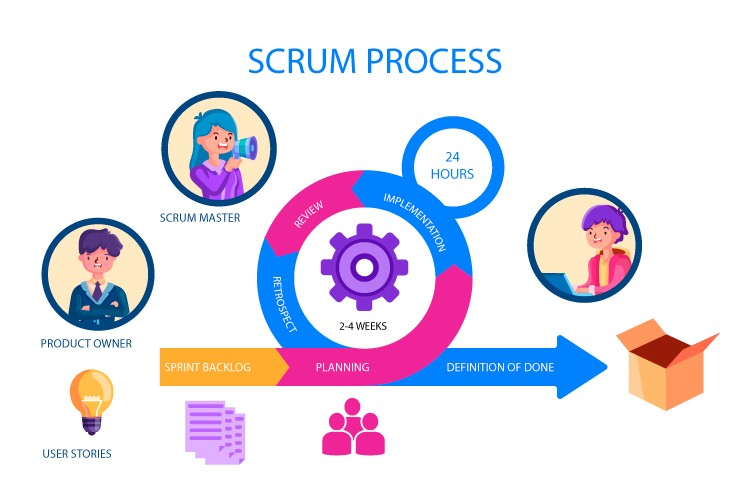
\includegraphics[width=10cm]{Images/scrum.jpg}
          \caption{Scrum Methodology}        
        \end{figure}
        \section{Conclusion}
          To sum up, I started with introducing the host company and descriping the internship. Then I moved to a project overview where I made a study about the solution currently implemented by the company to show its weeknesses and limitations. Finally I introduced and explained the methodology I will implement in this project.
          
    
    
    \newpage 
        \chapter{Litterature Review}






















  \end{document}
